%%%%%%%%%%%%%%%%%%%%%%%%%%%%%%%%%%%%%%%%%%%%%%%%%%%%%%%%%%%%%%%%%%%%%%%
%% Zusammenfassung und Ausblick
\section{Implementierung}
\label{sec:impl}

In diesem Kapitel werden einige Aspekte der Entwicklung aufgegriffen und im Detail ausgeführt. Der Name Implementierung bezieht sich nicht auf die Programmierung, sondern die Umsetzung von Schnittstellen und den Algorithmen hinter speziellen Problemen. So wird zum Beispiel in dem Unterkapitel \ref{sec:impl-rs} auf die Bewegung auf einer linearen Trajektorie eingegangen. Außerdem werden Probleme beschrieben und gelöst, die während der Umsetzung der Konzepte auftraten. Des Weiteren werden die genutzten Bibliotheken erwähnt und die Anbindung von ROS an die Konzepte. Den zentralen Aspekt in diesem Kapitel stellt jedoch Unterkapitel \ref{sec:impl-hop} dar. In diesem wird die Bestimmung für die Übergabeposition vorgestellt.

\subsection{Robotersteuerung - RATSYoubot \& RATSDummy \& RATSRose}
\label{sec:impl-rs}
In diesem Kapitel wird die Ansteuerung für die Roboter und deren Arme vorgestellt. Diese beruht vor allem auf der Kuka API für den Youbot. Außerdem wird die Bewegung auf einer linearen Trajektorie, sowie die einzelnen Aktionen die ein Roboter ausführen kann kurz aufgelistet und beschrieben.

\subsubsection{Ansteuerung der Aktoren}
\label{sec:impl-res-ak}
Die Aktoren innerhalb der Roboter werden mit Hilfe von ROS Topics angesteuert. Diese werden von dem Controllernode \textit{youbot\_driver} ausgelesen und in die Steuersignale für die Motoren umgewandelt. Für die Ansteuerung des Arms existieren zwei Topics. Der \textit{velocity\_command}-Topic erwartet für jedes Gelenk eine Geschwindigkeitsangabe. Für diese Arbeit wird jedoch mit Positionsangaben gearbeitet. Der dazu gehörige Topic \textit{arm\_controller/position\_command} benötigt ein Array mit Gelenkkonfigurationen. Dafür wird die ROS-Bibliothek \textit{BRICS} genutzt. Diese beinhaltet Nachrichten für inverse Kinematiken, wie zum  Beispiel: Posen, Vektoren und Rotationen im Kartesischen Raum oder Aktoren Nachrichten, wie Gelenkeinstellung, Gelenkgeschwindigkeiten und Gelenkbeschleunigungen. Neben der Armansteuerung gibt es für die Gripper eine eigene Topic \textit{gripper\_controller/position\_command}. Dieser transportiert ebenfalls Gelenkeinstellungen. Dabei kann die Position der einzelnen Finger des Grippers angegeben werden. Die Werte entsprechen dabei der Distanz der Finger zu ihrer Basisposition. Ein Nachteil der Ansteuerung über die Topics ist das fehlende Feedback. Der Absender erfährt nicht, ob das Signal angekommen ist und wann die Bewegung beendet ist. Sollen Bewegungen seriell ausgeführt werden muss der ausführende Thread blockiert werden, bis die Gelenke die Zielkonfiguration erreicht haben.  Ein paralleler Thread liest die aktuelle Gelenkkonfiguration aus und berechnet eine Differenz für jedes einzelne Gelenk und die Quadratsumme über alle Gelenke. Solange die Differenz für mindestens ein Gelenk oder die Summe der Quadrate ihre Schwellwerte überschreiten blockiert ein Mutex den ausführenden Thread. Ein weiteres Problem während der Implementierung stellte die Ungenauigkeit der Ansteuerung dar. Dabei kam es großen Abweichungen an einem Gelenk, wenn es eine große Winkeländerung hatte. Dieses Überschlagen lässt sich auf die Massenträgheit des Armes und dem abrupten Abbremsen der Motoren zurückführen. Dies konnte jedoch auch durch den parallelen Thread abgefangen werden. Dieser überprüft nun auch neben der Distanz zu der Zieleinstellung, die Distanz zur letzten gemessenen Gelenkeinstellung. Ist diese nahe null, also der Arm nicht mehr in Bewegung, und die Distanz zum Ziel zu groß wurde nochmal die selbe Gelenkeinstellung an den Motorencontroller geschickt.

Die Ansteuerung der mobilen Plattform wird mit einer einzelnen Topic \textit{cmd\_vel} umgesetzt. Dabei wird eine einzelne Nachricht übermittelt. Diese beinhaltet eine Twist Nachricht aus dem \textit{geometry\_msg} Paket. In dieser Nachricht kann eine lineare und eine Winkelgeschwindigkeit angegeben werden. Diese können für die einzelnen Achsen zerlegt werden. Für die mobile Plattform werden jedoch nur die X- und Y- Achsen der linearen, sowie die Z-Achse der Rotationsgeschwindigkeit ausgelesen und als absoluten Wert gesetzt. Der Controller rechnet anschließend die benötigten Steuersignale für die einzelnen Räder und Motoren aus.

\subsubsection{Lineare Bahnbewegung}
\label{sec:impl-res-lb}
Die lineare Bahnbewegung wird beim Aufheben, Ablegen und während der Übergabe benötigt. Dies liegt vor allem an der Kollisionsvermeidung des Objektes mit der Umwelt. Da die inverse Kinematik die Gelenkeinstellungen und nicht die Gelenkgeschwindigkeiten berechnet ist es nicht so einfach auf einer gezielten Trajektorie entlang zufahren. Der Übergang zwischen zwei Gelenkeinstellung wird nicht genau definiert. Wie in Abbildung \ref{fig:traj} dargestellt kommt es dabei durch unterschiedliche Gelenkgeschwindigkeiten zu einem Ausschlagen des Greifers. Je größer die Distanz zwischen zwei Posen, desto größer der Ausschlag. Deshalb kann dies verhindert beziehungsweise minimiert werden, indem Zwischenposen auf der Trajektorie ermittelt werden, die nacheinander angefahren werden. Dies erfordert zwar eine häufiges Aufrufen der inversen Kinematik, dafür kann eine Trajektorie mit einem geringen Ausschlag entlang gefahren werden. Tests mit dem YouBot Armen und der inversen Kinematik ergaben eine Distanz von 5 Millimetern zwischen den Zwischenposen als optimal. Bei einer kleineren Distanz reduzierte sich die Amplitude des Ausschlages weniger als vorher und steigert die Kosten durch einen häufigeren Aufruf der inversen Kinematik. Bei der Implementierung nutzt dafür vor allem die Orocos KDL Api, die auch bei der Implementierung der inversen Kinematik genutzt wird. Diese ermöglicht das Rechnen mit geometrischen Primitiven, so wurde der \lstinline|KDL::Frame| für die Abbildung von Koordinatensystemen und Posen genutzt. Dieser ermöglicht unter anderem die Bestimmung der Zwischenposen.

\begin{figure}[h]
	\centering
	\subfigure[]{%
		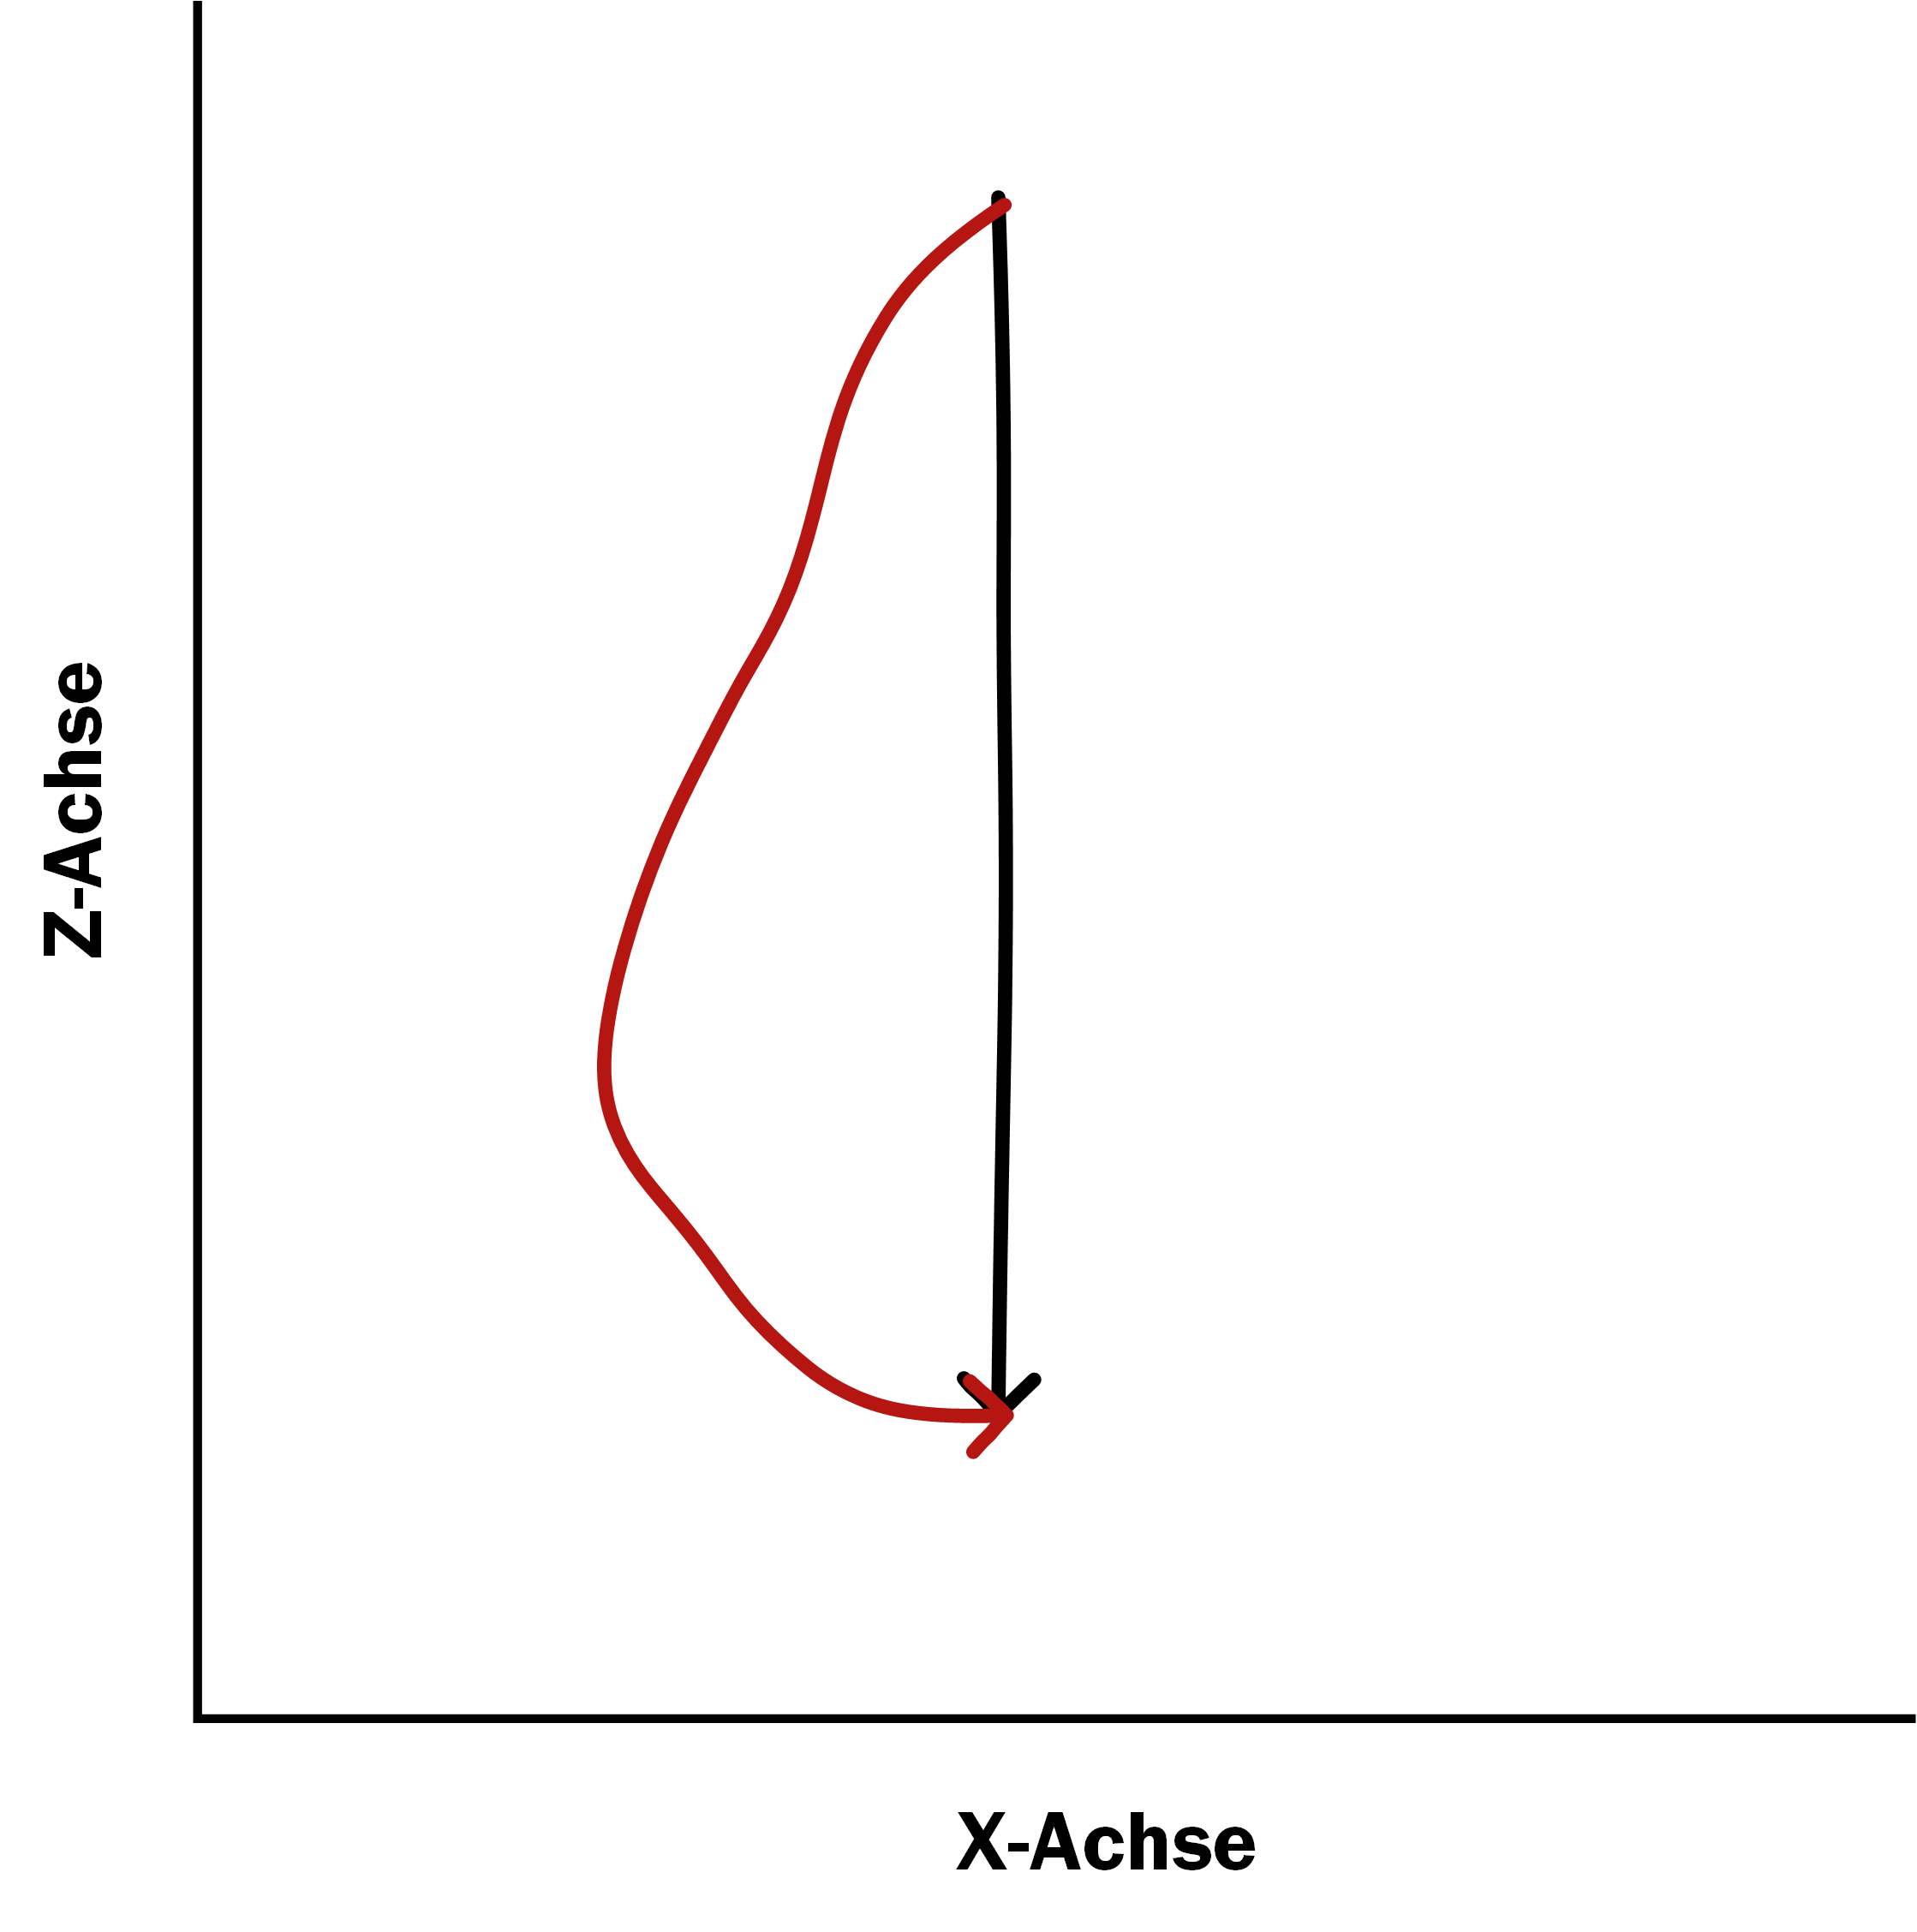
\includegraphics[scale=0.7]{fig/traj1}}
	\hfill
	\subfigure[]{%
		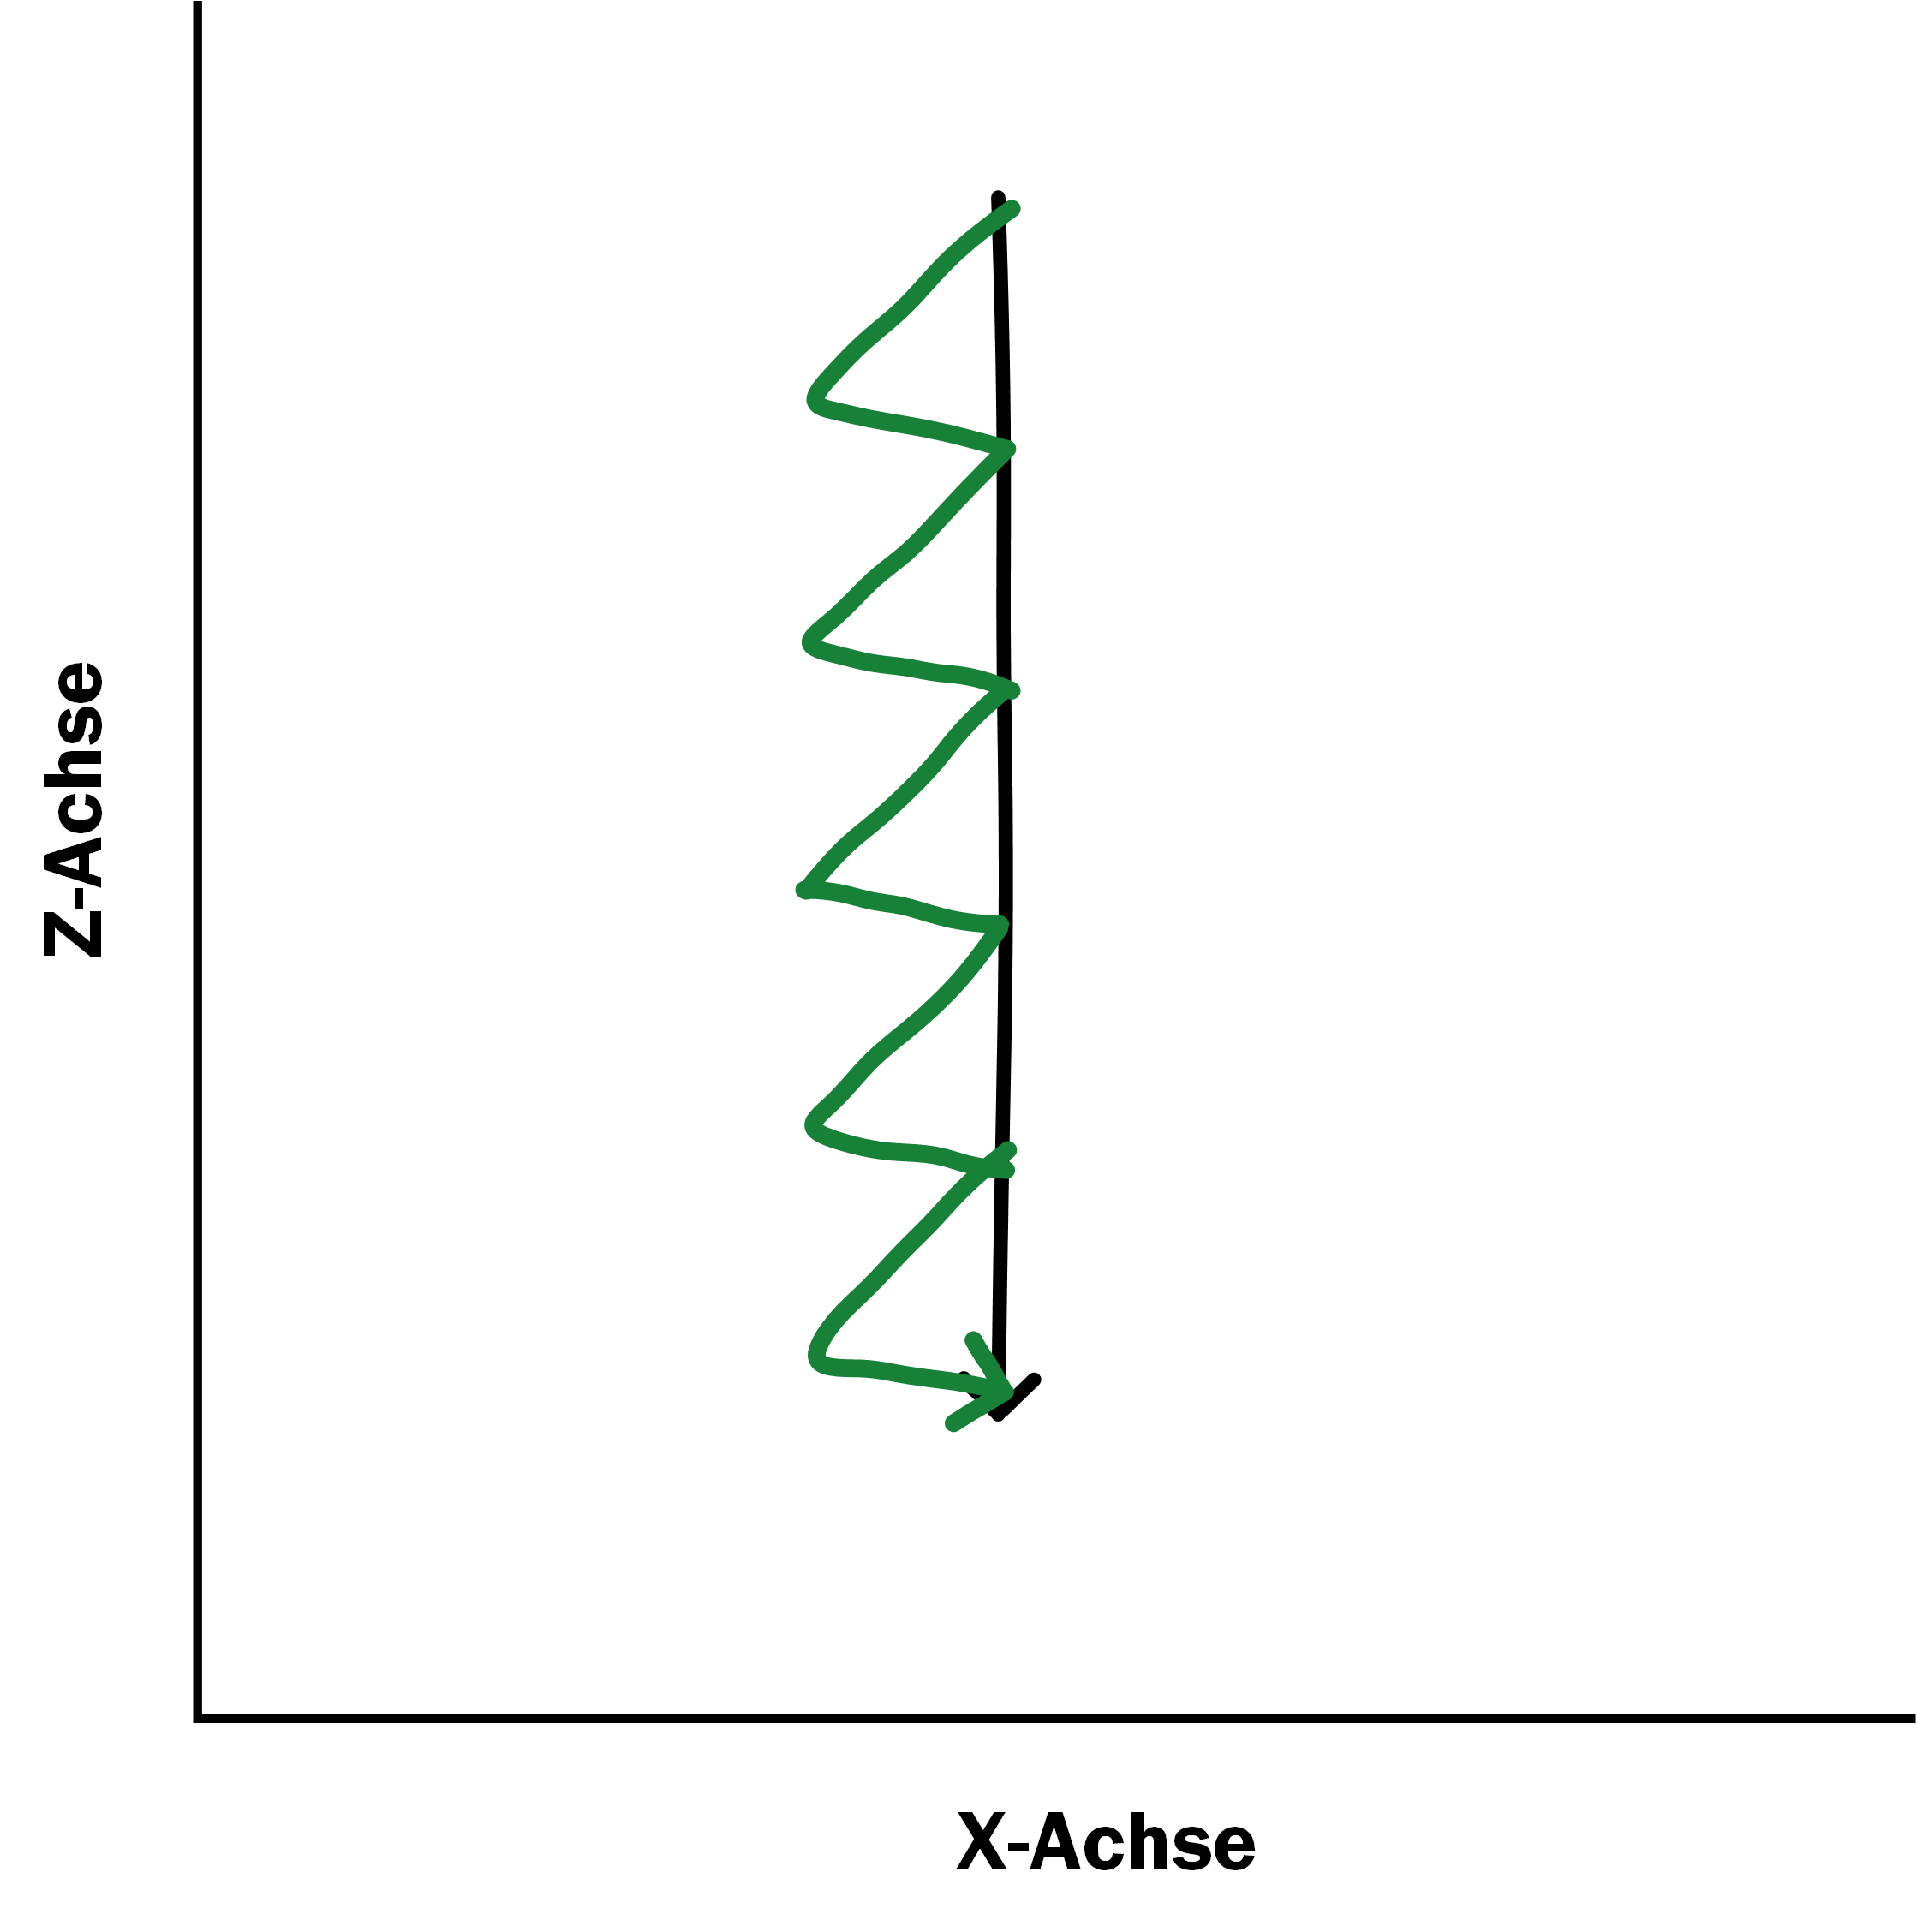
\includegraphics[scale=0.7]{fig/traj2}}
	\caption[Trajektorien des Greifers]{Die dargestellten Graphen stellen die gewünschte Trajektorie (schwarz) und die realen Trajektorien des Greifers dar. Dabei handelt es sich um eine lineare Absenkung auf der Z-Achse. Links: Trajektorie (rot) bei Angabe der Zielpose. Rechts: Trajektorie (grün) bei Angabe von Zwischenposen auf der gewünschten Trajektorie. Bildquelle: \cite{muggler2013torque}}	
	\label{fig:traj}
\end{figure}

\subsubsection{Aktionen der Roboter}

In diesem Unterkapitel wird sehr kurz auf die Aktionen eingegangen, die für die Roboter implementiert wurden. Aus Gründen des Umfangs wird dabei auf Grafiken, wie zum Beispiel UML-Diagramme, verzichtet. Aktionen die nur für einen Roboter implementiert wurden, sind speziell gekennzeichnet.

\paragraph{Greifer öffnen und schließen} Diese Aktion sind eigentlich zwei. Für beide Roboter wurde eine Aktion für das Öffnen und eine für das Schließen implementiert. Beim Öffnen fahren die beiden Finger des Greifers auf ihre maximal Position. Beim Schließen fahren die beiden Finger auf die Nullstellung. Befindet sich ein Objekt im Greifer versuchen die Finger den Schluss. Da die Kraft des Greifers jedoch nicht reicht und die Finger nur auf Spindeln sitzen, befinden sich die Finger am Ende der Aktion nicht in der Nullstellung.

\paragraph{Greifer in Pose bringen} Bei dieser Aktion wird als Parameter die sechsdimensionale Pose benötigt. Diese kann sich im globalen, als auch im lokalen Koordinatensystem des Roboters befinden und muss als solche mit einem Flag gekennzeichnet sein. Bei der Aktion wird zunächst die Gelenkeinstellung durch die inverse Kinematik ermittelt und anschließend mit der Methodik aus Kapitel \ref{sec:impl-res-ak} angesteuert. Zwei Sonderfälle dieser Aktion wurden für die Bewegung in die \textit{Candle}- oder \textit{Fold}-Pose implementiert.

\paragraph{Greifer an eine Pose annähern} Mit der Annäherung ist in diesem Fall eine lineare Trajektorie entlang der Z-Achse des Greifers in der Endpose gemeint. Auch hier wird als Parameter die Zielpose im lokalen oder globalen Koordinatensystem benötigt. Aus dieser Pose wird ein Vektor bestimmt. Dieser läuft entlang der Z-Achse der Greifers und hat eine Länge von vier Zentimetern. Entsprechend der Entwicklung aus Kapitel \ref{sec:impl-res-lb} werden acht Posen im fünf Millimeter Abstand auf diesem Vektor bestimmt und nacheinander angefahren.

\paragraph{Objekt aufheben} Diese Aktion ist eine Task, bei der seriell Aktionen ausgeführt werden. Als Parameter wird die Position des Zielobjektes benötigt, diese kann als lokaler Kontext angegeben werden oder mit einem Zeiger auf das Objekt im globalen Kontext. Neben der Position des Objektes wird die Rotation um die Z-Achse des Objektes berücksichtigt, da die X-Achse des Greifers parallel zur X-Achse des Objektes liegen muss. Bei der Durchführung wird zunächst der Greifer in einem vier Zentimeter Abstand in Position gebracht. Anschließend wird Greifer geöffnet und an die Position des Objektes angenähert. Folgend wird der Greifer geschlossen und der Arm in die \textit{Candle}-Pose gebracht. Für Rose gibt es eine erweiterte Form dieser Aktion, dabei wird Kontakt zur Naherkennung aufgenommen, um das Objekt visuell zu lokalisieren. Diese Koordinierung wird genutzt, um den Arbeitsraum des Roboters an die Position des Objektes anzupassen.

\paragraph{Objekt ablegen} Ähnlich dem Aufheben ist auch diese Aktion eine Task. Im Gegensatz dazu werden die Aktionen in einer anderen Reihenfolge ausgeführt. So fährt der Greifer zunächst in eine Pose etwas über dem Ziel. Öffnet anschließend die Finger um sich abschließend von dem Objekt zu entfernen. Dies geschieht auf einer linearen Trajektorie um das Objekt nicht zu verschieben. Abschließend bewegt der Arm sich in die \textit{Candle}-Pose.

\paragraph{Position einnehmen}
Diese Aktion betrifft nur Rose. Dabei fährt die mobile Plattform an eine neue Position. Dafür wird als Parameter eine X- und Y-Koordinate im globalen Koordinatensystem benötigt. Es werden keine rotierenden Bewegungen ausgeführt. Damit bleibt die Ausrichtung der Plattform gleich. Zur Lokalisierung wird dabei eine Mischung aus SLAM und Odometriedaten genutzt (siehe \ref{sec:impl-lopo}).

\paragraph{Übergabe} Die Übergabe ist die zentrale Aktion dieser Arbeit. Der Ablauf dieser ist bereits in Kapitel \ref{fun:han} und in den Abbildungen \ref{fig:gripper1}, \ref{fig:gripper2} und \ref{fig:gripper3} erläutert. Die Koordinierung dieser Aufgabe wird durch den RATSCore abgebildet. Die Positionsbestimmung kann durch eine direkte Koordinierung zwischen den Robotern stattfinden.

\subsection{Raumüberwachung - RATSHawk}
Die Raumüberwachung übernimmt die Detektion und Lokalisierung von Objekten im Raum. Dazu dient eine XTion-Kamera die an der Wand angebracht ist. Für das MRS wurde dafür ein eigener RATSMember, der RATSHawk, geschaffen. Momentan besitzt dieser Agent nur eine einzige Aktion: ein Objekt anhand seiner Farbe im Raum zu detektieren und die Position im globalen Kontext zu bestimmen. Als Parameter wird dafür ein Zeiger auf das gesuchte Objekt im globalen Kontext benötigt. Die Informationen über die Farbwerte des Objektes im HSV-Farbraum müssen im globalen Kontext unter dem Objekt abgelegt sein. Nach Ausführung der Aktion wird im Erfolgsfall die Position des Objektes in den globalen Kontext eingetragen. Die folgenden Kapitel befassen sich mit der verwendeten API \textit{Point Cloud Library} und den Subsequenzen zur Detektion und Lokalisierung des Objektes.

\subsubsection{PCL \& ROS}
Für die Anbindung der Kamerasysteme an ROS existieren die Pakete OpenNI2 und OpenNI2Launch. Diese generieren aus den Bildern der XTions Punktwolken, die mit Hilfe von Topics empfangen werden können. Für die Weiterverarbeitung der Punktwolken wird in dieser Arbeit die Point Cloud Library (PCL) genutzt. Diese bietet unter anderem verschiedene Filter, Feature und Keypoint Detektion, sowie Segmentierungen und Erkennungen. Einziges Problem ist Konvertierung der einzelnen Punktwolken-Formate. Jedoch stellt die PCL-API Methoden zur Umwandlung bereit. Dabei muss jedoch die Art der Punktwolke, zum Beispiel chlorierte Punktwolke (XYZRGB) oder Intensität-Punktwolke (XYZI), berücksichtigt werden. Für die XTion Kamerasysteme können entweder XYZ-Punktwolken ohne Farbwerte oder XYZRGB-Punktwolken mit Farbwerten im RGB-Farbraum genutzt werden.

\subsubsection{Detektion}
Die Detektion in dieser Arbeit basiert auf den Farb- und Geometriemerkmalen des Objektes. Dazu sind mehrere Schritte nötig. Nach der Konvertierung der Punktwolke wird zunächst TODO

\subsubsection{Lokalisierung}
Nachdem die Punktwolke für das Objekt extrahiert wurde, wird nun die Position und Rotation des Objektes bestimmt. Dafür wird zunächst eine Oriented Bounding Box (OBB) für das Objekt bestimmt. Eine Oriented Bounding Box entspricht einer Axis Aligned Bounding Box (AABB) die an den Eigenvektoren der Punktwolken orientiert ist. Eine Bounding Box entspricht einem Quader, in dem alle Punkte der Punktwolke enthalten sind. Die AABB ist an den Achsen des Koordinatensystem ausgerichtet. Für die Bestimmung der einzelnen Merkmale existiert in der PCL-API bereits ein vorgefertigter Algorithmus. Mit Hilfe diesem lässt sich neben dem minimalen und maximalen Punkt der Punktwolke auch der Mittelpunkt und die Rotationsmatrix für die OOB bestimmen. An Hand der Daten der OOB wird nun nochmal ein Abgleich der Geometrischen Eigenschaften des Objektes gemacht, dabei wird das Seitenverhältnis mit den hinterlegten Daten verglichen. Stimmen diese überein, wird aus der Kamerapose im globalen Koordinatensystem und der Objektpose im Kamera-Koordinatensystem die Objektpose im globalen Koordinatensystem berechnet. Jedoch zeigte ein Vergleich zwischen der realen und der berechneten Position Differenzen. Eigene Tests zeigten, dass die Differenzen Positionen bezogen sind. Die Ursache davon liegt vermutlich bei einer Verzerrung der Kameralinse oder einem fehlerhaften Parameter beim Registrierung der RGB-Bilder auf das IR-Bild. Um diese Verzerrung zu korrigieren wird nun ein Ausgleich-Modell verwendet, dass auf den gemessenen Testdaten beruht. Dazu wird zunächst auf dem Mittelpunkt des Kamerabildes der Normalenvektor der Kameraebene gesetzt und der Schnittpunkt mit der planaren Ebene des Bodens bestimmt. Anschließend wird die Distanz in der X- und Y- Richtung der Bildebene zum Objekt bestimmt und je nach Richtung mit einem Korrekturfaktor multipliziert. Diese Korrektur erbringt eine Genauigkeitssteigerung, sodass die Positionsbestimmung eine Genauigkeit von fünf Zentimetern erreicht. 

\subsection{Nahfelderkennung - RATSEye}
Im Gegensatz zur Raumüberwachung sitzt die Kamera nicht an der Wand, sondern am Roboter direkt. Dies betrifft in diesem Fall Rose. Die Nahfelderkennung ist als selbstständiger RATSMember, dem RATSEye, umgesetzt. Genau wie der RATSHawk besitzt das RATSEye nur eine Aktion zur farbbasierten Detektion und Lokalisierung. Aufgrund des geringen Abstandes zum Objekt hat dieser Agent gegenüber dem RATSHawk Vor- aber auch Nachteile. Auf der einen Hand ist die Genauigkeit der Ergebnisse auf dieser Distanz viel höher. Auch notwendige Korrekturen, wie beim RATSHawk, sind nicht nötig. Auf der anderen Hand benötigt der Agent die Vorarbeit eines anderen Agenten um arbeiten zu können. Da die Kamera am Arm von Rose angebracht ist, muss dieser erst in die \textit{Candle}-Pose gebracht werden. dies erhöht den Koordinierungsaufwand. Ein weitere Nachteil ist die schlechte Hardware, die dem Agenten zur Verfügung steht. Dadurch, dass die Kamera an den eingebauten Rechner in der mobilen Plattform gebunden ist, dauern Auswertungen der Punktwolken länger. Außerdem ist durch die Belastung des Systems eine Verzögerung der Punktwolken gegeben. Da die Berechnung für das Hardwaresystem belastend sind wird von einer wiederholenden Ausführung abgesehen und die Aktion nur bei Bedarf ausgeführt. Dies und die Verzögerung kann dazu führen, dass die Daten nicht dem aktuellen Ausschnitt entspricht, an dem sich der Agent befindet. Um dies zu umgehen wurde ein paralleler Thread aufgebaut. Dieser empfängt die Punktwolken und legt die aktuellste in einem Speicher ab. Wird nun die Hauptfunktion ausgeführt blockiert diese ihren eigenen Thread mit einem Mutex. Der Datenthread hebt diese Sperre auf, sobald eine neues Punktwolke im Speicher liegt. Daraufhin blockiert der Hauptthread den Datenthread mit einem weiteren Mutex. Dies ist nötig, da während der Analyse neue Punktwolken eintreffen könnten und den Speicher überschreiben würden. Nach der Detektion und Lokalisierung wird diese Sperre wieder aufgehoben. Die Detektion und Lokalisierung laufen genauso ab, wie bei der Raumüberwachung. Nur die Korrektur der Lokalisierung ist nicht nötig.

Während der Testphase kam es bei der Nahfelderkennung zu zunächst unerklärlichen temporären Problemen. Dabei konnte das Objekt nicht detektiert werden. Dies lies sich auf zu kleine Punktwolken zurückführen. Eine Inspektion der aufgenommenen Bilder ergab, dass einzelne Bilder sehr dunkel waren. Bei einer genaueren Untersuchen stellte sich heraus, dass Reflexionen der Beleuchtung durch die spiegelnde Oberfläche der mobilen Plattform direkt in die Kamera blendeten. Diese führte einen automatischen Helligkeitsausgleich durch und verdunkelte das komplette Bild. Diese Problem konnte mechanisch umgangen werden, indem die spiegelnde Fläche mit schwarzem Klebeband verdeckt wurde.
\subsection{Koordinierung - RATSCore \& RATSMember}
\subsection{Lokale Positionierung}
\label{sec:impl-lopo}
\subsection{Handoverpoint}
\label{sec:impl-hop}
